%!TEX root = ../tfe.tex
\section*{Test case to assess the implementation of the overturner model}
This note is an adaptation of Eric Deleersnijder's working paper \cite{deleersnijder2011test}.

\subsection*{Governing equations}
Let us consider a water domain, whose width is denoted $B(t,\b{x})$, where $t$ is the time and $\b{x} = (y,z)$ is the position vector. The continuity equation is
\begin{equation} \label{eq:testcase:continuity}
	\frac{\partial B}{\partial t} + \nabla \cdot (B\b{u}) = 0,
\end{equation}
where $\b{u}(t,\b{x})$ is the latitudinally-averaged meridional velocity. Assuming that mixing along the parallels is sufficiently efficient, we may study the concentration of a passive tracer by means of a two-dimensional model. The latitudinally-averaged concentration of the tracer $C(t,\b{x})$ obeys the following partial differential equation :
\begin{equation} \label{eq:testcase:conservative}
	\frac{\partial (BC)}{\partial t} + \nabla \cdot (B \b{u} C) = Q\delta(\b{x} - \b{x}_1) + \nabla \cdot (B\b{K} \cdot \nabla C), 
\end{equation}
where $\b{K}$ is the diffusivity tensor (symmetric and positive definite); $\delta$ is the Dirac delta function with $\delta(\b{x}-\b{x}_n) = \delta(x-x_n)\delta(y-y_n)$; $Q(t)$ is the rate of release of a lineic source on a segment of length $B$ along the latitude direction located at $\b{x} = \b{x}_1$. If $C(t,\b x)$ represents the 
density of the tracer in water, then $Q(t)$ is the mass of tracer released per second by the source.

Equation \eqref{eq:testcase:conservative} is the so-called conservative form of the model. The convective form is obtained by combining equations \eqref{eq:testcase:continuity} and \eqref{eq:testcase:conservative}:
\begin{equation}  \label{eq:testcase:convective}
	\frac{\partial C}{\partial t} + \b{u} \cdot \nabla C = \frac{Q}{B} \delta(\b{x} - \b{x}_1) + \frac{1}{B} \nabla \cdot (B\b{K} \cdot \nabla C).
\end{equation}

\subsection*{An idealised model}
% Recall that we are building a test case for assessing the validity of our implementation of the overturner model.
Now we make some simplifying assumptions which will allow us to build an analytical solution. First, we consider an infinite domain, i.e.
\begin{equation} \label{eq:testcase:domain}
	-\infty < y < \infty, \ -\infty < z < \infty.
\end{equation}
We assume a constant width $B$ and a constant velocity field
\begin{equation} \label{eq:testcase:velocity}
	\b{u}(t,\b{x}) = v \b e_y + w \b e_z,
\end{equation}
where $\b e_y$ and $\b e_z$ are the unit vectors associated respectively with the $y$- and $z$-coordinate axis. Furthermore, the diffusivity tensor is supposed constant and diagonal :
\begin{equation} \label{eq:testcase:diffusivity}
	\b{K} = \begin{pmatrix}
			K_{yy} & 0 \\
			0 & K_{zz}
			\end{pmatrix},	
\end{equation}
where $K_{yy},\ K_{zz} > 0$. Finally, we consider a sudden pointwise release of tracer at $t=0$. Hence, $Q(t)$ is of the form :
\begin{equation}
	Q(t) = M\delta(t),
\end{equation} 
where $M$ is the mass of tracer released at $t=0$.

Under these assumptions, equation \eqref{eq:testcase:convective} simplifies to :
\begin{equation} \label{eq:testcase}
	\frac{\partial C}{\partial t} + v \frac{\partial C}{\partial y} + w \frac{\partial C}{\partial z} = \frac{M}{B} \delta(t) \delta(y - y_1)\delta(z-z_1) + K_{yy} \frac{\partial^2 C}{\partial y^2} + K_{zz} \frac{\partial^2 C}{\partial z^2}.
\end{equation}
For the sake of simplicity, we can forget about the fact that our model is width-integrated and consider that it is a purely two-dimensional model with a point-source
\begin{equation}
	Q := J\delta(t),
\end{equation}
where $J := M/B$ can be regarded as the mass of tracer released by the sudden point source at $\b x = \b x_1$, if $C$ now represents the two-dimensional density (i.e., in [$kg/m^2$]) of the tracer in water.\footnote{This could be a bit confusing. As we switch from a 3-dimensional interpretation of the model to a 2-dimensional one, the meaning of the parameters changes. Hence, in the 3-dimensional interpretation, $C$ represents a 3D density ([$kg/m^3$]) and $M$ is a mass, whereas in the 2-dimensional interpretation, $C$ is a 2D density ([$kg/m^2$]) and $M$ has units of [$kg\;m$].} This is represented on figure \ref{fig:testcase_scheme}. \textcolor{red}{On peut aussi simplement considérer B = 1. Attention, si on opte finalement pour cette option, un facteur B doit être présent pour le calcul de certains diagnostiques.}
\begin{figure}[H]
	\centering
 	\begin{subfigure}[b]{0.48\textwidth}
        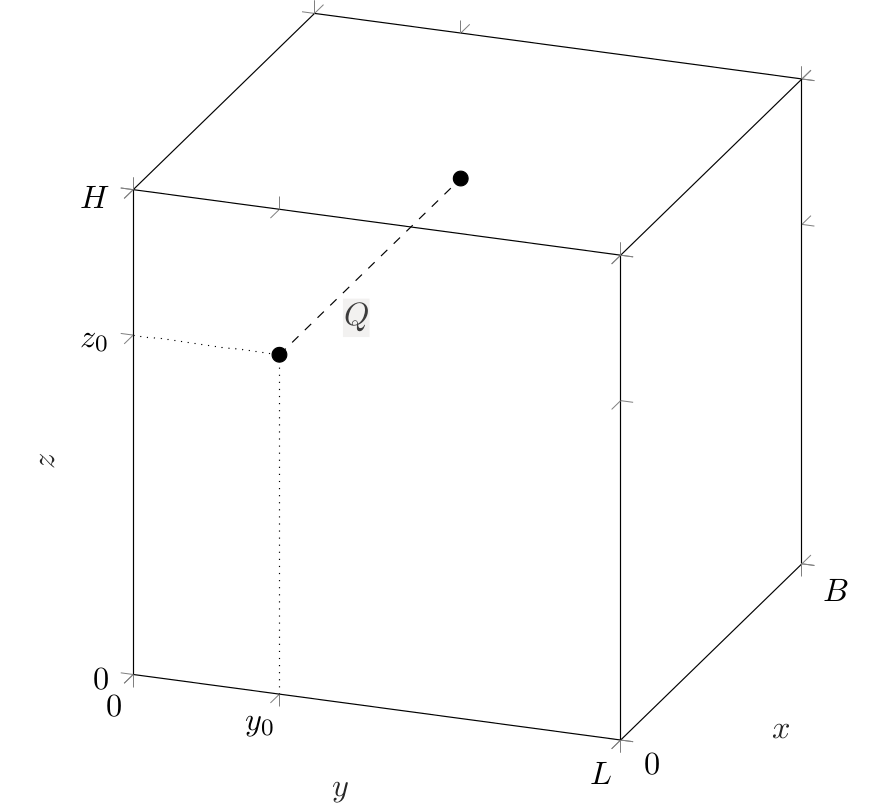
\includegraphics[width=\textwidth]{fig/testcase_scheme3D.png}
        \caption{3D interpretation of the model.}
        \label{fig:testcase_scheme3D}
    \end{subfigure}
	\begin{subfigure}[b]{0.48\textwidth}
        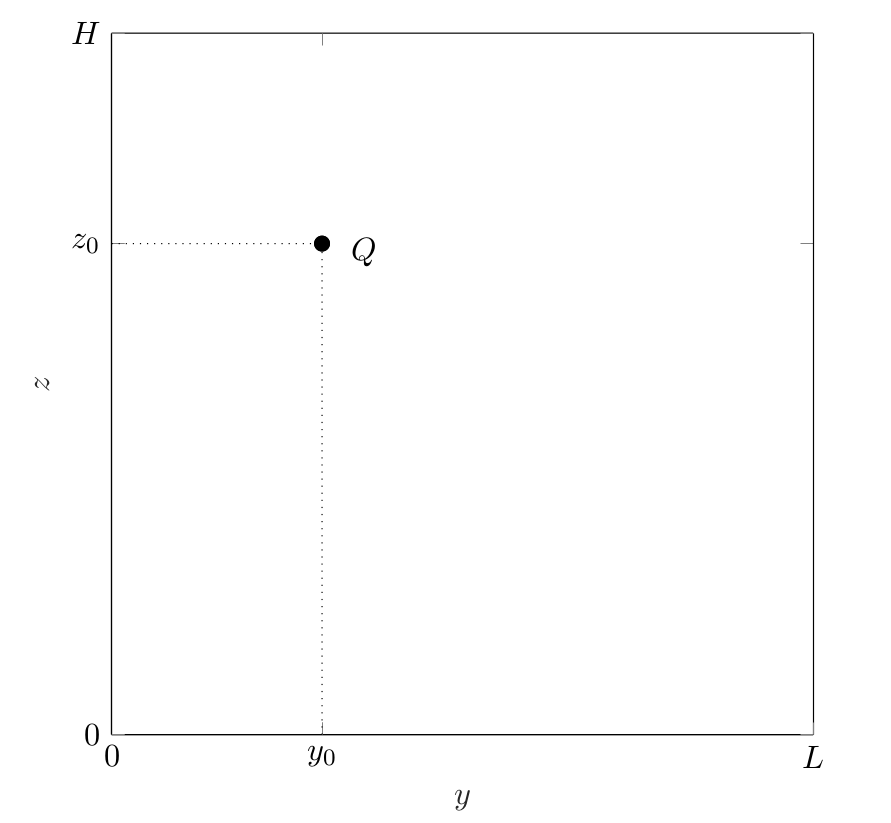
\includegraphics[width=\textwidth]{fig/testcase_scheme2D.png}
        \caption{2D interpretation of the model.}
        \label{fig:testcase_scheme2D}
    \end{subfigure}
    \caption{Illustration of the 3D and 2D interpretations of the model.}
    \label{fig:testcase_scheme}
\end{figure}

% This file was created by matlab2tikz.
%
%The latest updates can be retrieved from
%  http://www.mathworks.com/matlabcentral/fileexchange/22022-matlab2tikz-matlab2tikz
%where you can also make suggestions and rate matlab2tikz.
%
\begin{tikzpicture}

\begin{axis}[%
width=0.307\textwidth,
height=0.333\textwidth,
at={(0\textwidth,0\textwidth)},
scale only axis,
plot box ratio=1 1 1,
xmin=0,
xmax=1,
xtick={0,1},
xticklabels={{0},{$B$}},
tick align=outside,
xlabel style={font=\color{white!15!black}},
xlabel={$x$},
ymin=0,
ymax=1,
ytick={0.3},
yticklabels={{$y_0$}},
ylabel style={font=\color{white!15!black}},
ylabel={$y$},
zmin=0,
zmax=1,
ztick={0.7},
zticklabels={{$z_0$}},
zlabel style={font=\color{white!15!black}},
zlabel={$z$},
view={69.6}{-21.2},
axis background/.style={fill=white}
]
\addplot3 [color=black, dotted]
 table[row sep=crcr] {%
0	0.3	0\\
0	0.3	0.00707070707070707\\
0	0.3	0.0141414141414141\\
0	0.3	0.0212121212121212\\
0	0.3	0.0282828282828283\\
0	0.3	0.0353535353535354\\
0	0.3	0.0424242424242424\\
0	0.3	0.0494949494949495\\
0	0.3	0.0565656565656566\\
0	0.3	0.0636363636363636\\
0	0.3	0.0707070707070707\\
0	0.3	0.0777777777777778\\
0	0.3	0.0848484848484848\\
0	0.3	0.0919191919191919\\
0	0.3	0.098989898989899\\
0	0.3	0.106060606060606\\
0	0.3	0.113131313131313\\
0	0.3	0.12020202020202\\
0	0.3	0.127272727272727\\
0	0.3	0.134343434343434\\
0	0.3	0.141414141414141\\
0	0.3	0.148484848484848\\
0	0.3	0.155555555555556\\
0	0.3	0.162626262626263\\
0	0.3	0.16969696969697\\
0	0.3	0.176767676767677\\
0	0.3	0.183838383838384\\
0	0.3	0.190909090909091\\
0	0.3	0.197979797979798\\
0	0.3	0.205050505050505\\
0	0.3	0.212121212121212\\
0	0.3	0.219191919191919\\
0	0.3	0.226262626262626\\
0	0.3	0.233333333333333\\
0	0.3	0.24040404040404\\
0	0.3	0.247474747474747\\
0	0.3	0.254545454545455\\
0	0.3	0.261616161616162\\
0	0.3	0.268686868686869\\
0	0.3	0.275757575757576\\
0	0.3	0.282828282828283\\
0	0.3	0.28989898989899\\
0	0.3	0.296969696969697\\
0	0.3	0.304040404040404\\
0	0.3	0.311111111111111\\
0	0.3	0.318181818181818\\
0	0.3	0.325252525252525\\
0	0.3	0.332323232323232\\
0	0.3	0.339393939393939\\
0	0.3	0.346464646464646\\
0	0.3	0.353535353535354\\
0	0.3	0.360606060606061\\
0	0.3	0.367676767676768\\
0	0.3	0.374747474747475\\
0	0.3	0.381818181818182\\
0	0.3	0.388888888888889\\
0	0.3	0.395959595959596\\
0	0.3	0.403030303030303\\
0	0.3	0.41010101010101\\
0	0.3	0.417171717171717\\
0	0.3	0.424242424242424\\
0	0.3	0.431313131313131\\
0	0.3	0.438383838383838\\
0	0.3	0.445454545454545\\
0	0.3	0.452525252525252\\
0	0.3	0.45959595959596\\
0	0.3	0.466666666666667\\
0	0.3	0.473737373737374\\
0	0.3	0.480808080808081\\
0	0.3	0.487878787878788\\
0	0.3	0.494949494949495\\
0	0.3	0.502020202020202\\
0	0.3	0.509090909090909\\
0	0.3	0.516161616161616\\
0	0.3	0.523232323232323\\
0	0.3	0.53030303030303\\
0	0.3	0.537373737373737\\
0	0.3	0.544444444444444\\
0	0.3	0.551515151515151\\
0	0.3	0.558585858585859\\
0	0.3	0.565656565656566\\
0	0.3	0.572727272727273\\
0	0.3	0.57979797979798\\
0	0.3	0.586868686868687\\
0	0.3	0.593939393939394\\
0	0.3	0.601010101010101\\
0	0.3	0.608080808080808\\
0	0.3	0.615151515151515\\
0	0.3	0.622222222222222\\
0	0.3	0.629292929292929\\
0	0.3	0.636363636363636\\
0	0.3	0.643434343434343\\
0	0.3	0.65050505050505\\
0	0.3	0.657575757575757\\
0	0.3	0.664646464646465\\
0	0.3	0.671717171717172\\
0	0.3	0.678787878787879\\
0	0.3	0.685858585858586\\
0	0.3	0.692929292929293\\
0	0.3	0.7\\
};
 \addplot3 [color=black, dotted]
 table[row sep=crcr] {%
0	0	0.7\\
0	0.00303030303030303	0.7\\
0	0.00606060606060606	0.7\\
0	0.00909090909090909	0.7\\
0	0.0121212121212121	0.7\\
0	0.0151515151515152	0.7\\
0	0.0181818181818182	0.7\\
0	0.0212121212121212	0.7\\
0	0.0242424242424242	0.7\\
0	0.0272727272727273	0.7\\
0	0.0303030303030303	0.7\\
0	0.0333333333333333	0.7\\
0	0.0363636363636364	0.7\\
0	0.0393939393939394	0.7\\
0	0.0424242424242424	0.7\\
0	0.0454545454545455	0.7\\
0	0.0484848484848485	0.7\\
0	0.0515151515151515	0.7\\
0	0.0545454545454545	0.7\\
0	0.0575757575757576	0.7\\
0	0.0606060606060606	0.7\\
0	0.0636363636363636	0.7\\
0	0.0666666666666667	0.7\\
0	0.0696969696969697	0.7\\
0	0.0727272727272727	0.7\\
0	0.0757575757575758	0.7\\
0	0.0787878787878788	0.7\\
0	0.0818181818181818	0.7\\
0	0.0848484848484849	0.7\\
0	0.0878787878787879	0.7\\
0	0.0909090909090909	0.7\\
0	0.0939393939393939	0.7\\
0	0.096969696969697	0.7\\
0	0.1	0.7\\
0	0.103030303030303	0.7\\
0	0.106060606060606	0.7\\
0	0.109090909090909	0.7\\
0	0.112121212121212	0.7\\
0	0.115151515151515	0.7\\
0	0.118181818181818	0.7\\
0	0.121212121212121	0.7\\
0	0.124242424242424	0.7\\
0	0.127272727272727	0.7\\
0	0.13030303030303	0.7\\
0	0.133333333333333	0.7\\
0	0.136363636363636	0.7\\
0	0.139393939393939	0.7\\
0	0.142424242424242	0.7\\
0	0.145454545454545	0.7\\
0	0.148484848484848	0.7\\
0	0.151515151515152	0.7\\
0	0.154545454545455	0.7\\
0	0.157575757575758	0.7\\
0	0.160606060606061	0.7\\
0	0.163636363636364	0.7\\
0	0.166666666666667	0.7\\
0	0.16969696969697	0.7\\
0	0.172727272727273	0.7\\
0	0.175757575757576	0.7\\
0	0.178787878787879	0.7\\
0	0.181818181818182	0.7\\
0	0.184848484848485	0.7\\
0	0.187878787878788	0.7\\
0	0.190909090909091	0.7\\
0	0.193939393939394	0.7\\
0	0.196969696969697	0.7\\
0	0.2	0.7\\
0	0.203030303030303	0.7\\
0	0.206060606060606	0.7\\
0	0.209090909090909	0.7\\
0	0.212121212121212	0.7\\
0	0.215151515151515	0.7\\
0	0.218181818181818	0.7\\
0	0.221212121212121	0.7\\
0	0.224242424242424	0.7\\
0	0.227272727272727	0.7\\
0	0.23030303030303	0.7\\
0	0.233333333333333	0.7\\
0	0.236363636363636	0.7\\
0	0.239393939393939	0.7\\
0	0.242424242424242	0.7\\
0	0.245454545454545	0.7\\
0	0.248484848484848	0.7\\
0	0.251515151515152	0.7\\
0	0.254545454545455	0.7\\
0	0.257575757575758	0.7\\
0	0.260606060606061	0.7\\
0	0.263636363636364	0.7\\
0	0.266666666666667	0.7\\
0	0.26969696969697	0.7\\
0	0.272727272727273	0.7\\
0	0.275757575757576	0.7\\
0	0.278787878787879	0.7\\
0	0.281818181818182	0.7\\
0	0.284848484848485	0.7\\
0	0.287878787878788	0.7\\
0	0.290909090909091	0.7\\
0	0.293939393939394	0.7\\
0	0.296969696969697	0.7\\
0	0.3	0.7\\
};
 \addplot3 [color=black, dashed]
 table[row sep=crcr] {%
0	0.3	0.7\\
0.0101010101010101	0.3	0.7\\
0.0202020202020202	0.3	0.7\\
0.0303030303030303	0.3	0.7\\
0.0404040404040404	0.3	0.7\\
0.0505050505050505	0.3	0.7\\
0.0606060606060606	0.3	0.7\\
0.0707070707070707	0.3	0.7\\
0.0808080808080808	0.3	0.7\\
0.0909090909090909	0.3	0.7\\
0.101010101010101	0.3	0.7\\
0.111111111111111	0.3	0.7\\
0.121212121212121	0.3	0.7\\
0.131313131313131	0.3	0.7\\
0.141414141414141	0.3	0.7\\
0.151515151515152	0.3	0.7\\
0.161616161616162	0.3	0.7\\
0.171717171717172	0.3	0.7\\
0.181818181818182	0.3	0.7\\
0.191919191919192	0.3	0.7\\
0.202020202020202	0.3	0.7\\
0.212121212121212	0.3	0.7\\
0.222222222222222	0.3	0.7\\
0.232323232323232	0.3	0.7\\
0.242424242424242	0.3	0.7\\
0.252525252525253	0.3	0.7\\
0.262626262626263	0.3	0.7\\
0.272727272727273	0.3	0.7\\
0.282828282828283	0.3	0.7\\
0.292929292929293	0.3	0.7\\
0.303030303030303	0.3	0.7\\
0.313131313131313	0.3	0.7\\
0.323232323232323	0.3	0.7\\
0.333333333333333	0.3	0.7\\
0.343434343434343	0.3	0.7\\
0.353535353535354	0.3	0.7\\
0.363636363636364	0.3	0.7\\
0.373737373737374	0.3	0.7\\
0.383838383838384	0.3	0.7\\
0.393939393939394	0.3	0.7\\
0.404040404040404	0.3	0.7\\
0.414141414141414	0.3	0.7\\
0.424242424242424	0.3	0.7\\
0.434343434343434	0.3	0.7\\
0.444444444444444	0.3	0.7\\
0.454545454545455	0.3	0.7\\
0.464646464646465	0.3	0.7\\
0.474747474747475	0.3	0.7\\
0.484848484848485	0.3	0.7\\
0.494949494949495	0.3	0.7\\
0.505050505050505	0.3	0.7\\
0.515151515151515	0.3	0.7\\
0.525252525252525	0.3	0.7\\
0.535353535353535	0.3	0.7\\
0.545454545454545	0.3	0.7\\
0.555555555555556	0.3	0.7\\
0.565656565656566	0.3	0.7\\
0.575757575757576	0.3	0.7\\
0.585858585858586	0.3	0.7\\
0.595959595959596	0.3	0.7\\
0.606060606060606	0.3	0.7\\
0.616161616161616	0.3	0.7\\
0.626262626262626	0.3	0.7\\
0.636363636363636	0.3	0.7\\
0.646464646464647	0.3	0.7\\
0.656565656565657	0.3	0.7\\
0.666666666666667	0.3	0.7\\
0.676767676767677	0.3	0.7\\
0.686868686868687	0.3	0.7\\
0.696969696969697	0.3	0.7\\
0.707070707070707	0.3	0.7\\
0.717171717171717	0.3	0.7\\
0.727272727272727	0.3	0.7\\
0.737373737373737	0.3	0.7\\
0.747474747474748	0.3	0.7\\
0.757575757575758	0.3	0.7\\
0.767676767676768	0.3	0.7\\
0.777777777777778	0.3	0.7\\
0.787878787878788	0.3	0.7\\
0.797979797979798	0.3	0.7\\
0.808080808080808	0.3	0.7\\
0.818181818181818	0.3	0.7\\
0.828282828282828	0.3	0.7\\
0.838383838383838	0.3	0.7\\
0.848484848484849	0.3	0.7\\
0.858585858585859	0.3	0.7\\
0.868686868686869	0.3	0.7\\
0.878787878787879	0.3	0.7\\
0.888888888888889	0.3	0.7\\
0.898989898989899	0.3	0.7\\
0.909090909090909	0.3	0.7\\
0.919191919191919	0.3	0.7\\
0.929292929292929	0.3	0.7\\
0.939393939393939	0.3	0.7\\
0.94949494949495	0.3	0.7\\
0.95959595959596	0.3	0.7\\
0.96969696969697	0.3	0.7\\
0.97979797979798	0.3	0.7\\
0.98989898989899	0.3	0.7\\
1	0.3	0.7\\
};
 \addplot3 [color=black, draw=none, mark size=2.5pt, mark=*, mark options={solid, black}]
 table[row sep=crcr] {%
0	0.3	0.7\\
};
 \addplot3 [color=black, draw=none, mark size=2.5pt, mark=*, mark options={solid, black}]
 table[row sep=crcr] {%
1	0.3	0.7\\
};
 \end{axis}

\begin{axis}[%
width=0.552\textwidth,
height=0.409\textwidth,
at={(-0.132\textwidth,-0.045\textwidth)},
scale only axis,
xmin=0,
xmax=1,
ymin=0,
ymax=1,
axis line style={draw=none},
ticks=none,
axis x line*=bottom,
axis y line*=left
]
\node[below right, align=left]
at (rel axis cs:0.4,0.63) {$Q$};
\addplot [color=black, dashed, forget plot]
  table[row sep=crcr]{%
0.646191646191646	0.654058043117745\\
0.718673218673219	0.64179104477612\\
};
\addplot [color=black, dashed, forget plot]
  table[row sep=crcr]{%
0.793611793611793	0.85140464344942\\
0.866093366093366	0.839137645107795\\
};
\addplot [color=black, dashed, forget plot]
  table[row sep=crcr]{%
0.796068796068795	0.307457711442787\\
0.868550368550368	0.295190713101162\\
};
\addplot [color=black, dashed, forget plot]
  table[row sep=crcr]{%
0.648648648648648	0.108452736318409\\
0.721130221130221	0.0961857379767835\\
};
\addplot [color=black, dashed, forget plot]
  table[row sep=crcr]{%
0.313267813267813	0.935981757877281\\
0.385749385749385	0.923714759535655\\
};
\addplot [color=black, dashed, forget plot]
  table[row sep=crcr]{%
0.164619164619164	0.740293532338309\\
0.237100737100737	0.728026533996684\\
};
\addplot [color=black, dashed, forget plot]
  table[row sep=crcr]{%
0.168304668304668	0.196346600331676\\
0.24078624078624	0.18407960199005\\
};
\addplot [color=black, dashed, forget plot]
  table[row sep=crcr]{%
0.23955773955774	0.808286898839139\\
0.23955773955774	0.724709784411278\\
};
\addplot [color=black, dashed, forget plot]
  table[row sep=crcr]{%
0.39066339066339	1.00895024875622\\
0.39066339066339	0.92537313432836\\
};
\addplot [color=black, dashed, forget plot]
  table[row sep=crcr]{%
0.793611793611793	0.937640132669985\\
0.793611793611793	0.854063018242124\\
};
\addplot [color=black, dashed, forget plot]
  table[row sep=crcr]{%
0.643734643734643	0.74029353233831\\
0.643734643734643	0.656716417910449\\
};
\addplot [color=black, dashed, forget plot]
  table[row sep=crcr]{%
0.239557739557739	0.184737976782754\\
0.239557739557739	0.101160862354894\\
};
\addplot [color=black, dashed, forget plot]
  table[row sep=crcr]{%
0.644963144963145	0.105135986733003\\
0.644963144963145	0.0215588723051426\\
};
\addplot [color=black, dashed, forget plot]
  table[row sep=crcr]{%
0.796068796068796	0.299165837479272\\
0.796068796068796	0.215588723051412\\
};
\end{axis}
\end{tikzpicture}%
% This file was created by matlab2tikz.
%
%The latest updates can be retrieved from
%  http://www.mathworks.com/matlabcentral/fileexchange/22022-matlab2tikz-matlab2tikz
%where you can also make suggestions and rate matlab2tikz.
%
\begin{tikzpicture}

\begin{axis}[%
width=0.333\textwidth,
height=0.333\textwidth,
at={(0\textwidth,0\textwidth)},
scale only axis,
plot box ratio=1 1 1,
xmin=0,
xmax=1,
xtick={0,1},
xticklabels={{0},{$B$}},
xlabel style={font=\color{white!15!black}},
xlabel={$x$},
ymin=0,
ymax=1,
ytick={0.3},
yticklabels={{$y_0$}},
ylabel style={font=\color{white!15!black}},
ylabel={$y$},
zmin=0,
zmax=1,
ztick={0.7},
zticklabels={{$z_0$}},
zlabel style={font=\color{white!15!black}},
zlabel={$z$},
view={90}{0},
axis background/.style={fill=white}
]
\addplot3 [color=black, dotted]
 table[row sep=crcr] {%
0	0.3	0\\
0	0.3	0.00707070707070707\\
0	0.3	0.0141414141414141\\
0	0.3	0.0212121212121212\\
0	0.3	0.0282828282828283\\
0	0.3	0.0353535353535354\\
0	0.3	0.0424242424242424\\
0	0.3	0.0494949494949495\\
0	0.3	0.0565656565656566\\
0	0.3	0.0636363636363636\\
0	0.3	0.0707070707070707\\
0	0.3	0.0777777777777778\\
0	0.3	0.0848484848484848\\
0	0.3	0.0919191919191919\\
0	0.3	0.098989898989899\\
0	0.3	0.106060606060606\\
0	0.3	0.113131313131313\\
0	0.3	0.12020202020202\\
0	0.3	0.127272727272727\\
0	0.3	0.134343434343434\\
0	0.3	0.141414141414141\\
0	0.3	0.148484848484848\\
0	0.3	0.155555555555556\\
0	0.3	0.162626262626263\\
0	0.3	0.16969696969697\\
0	0.3	0.176767676767677\\
0	0.3	0.183838383838384\\
0	0.3	0.190909090909091\\
0	0.3	0.197979797979798\\
0	0.3	0.205050505050505\\
0	0.3	0.212121212121212\\
0	0.3	0.219191919191919\\
0	0.3	0.226262626262626\\
0	0.3	0.233333333333333\\
0	0.3	0.24040404040404\\
0	0.3	0.247474747474747\\
0	0.3	0.254545454545455\\
0	0.3	0.261616161616162\\
0	0.3	0.268686868686869\\
0	0.3	0.275757575757576\\
0	0.3	0.282828282828283\\
0	0.3	0.28989898989899\\
0	0.3	0.296969696969697\\
0	0.3	0.304040404040404\\
0	0.3	0.311111111111111\\
0	0.3	0.318181818181818\\
0	0.3	0.325252525252525\\
0	0.3	0.332323232323232\\
0	0.3	0.339393939393939\\
0	0.3	0.346464646464646\\
0	0.3	0.353535353535354\\
0	0.3	0.360606060606061\\
0	0.3	0.367676767676768\\
0	0.3	0.374747474747475\\
0	0.3	0.381818181818182\\
0	0.3	0.388888888888889\\
0	0.3	0.395959595959596\\
0	0.3	0.403030303030303\\
0	0.3	0.41010101010101\\
0	0.3	0.417171717171717\\
0	0.3	0.424242424242424\\
0	0.3	0.431313131313131\\
0	0.3	0.438383838383838\\
0	0.3	0.445454545454545\\
0	0.3	0.452525252525252\\
0	0.3	0.45959595959596\\
0	0.3	0.466666666666667\\
0	0.3	0.473737373737374\\
0	0.3	0.480808080808081\\
0	0.3	0.487878787878788\\
0	0.3	0.494949494949495\\
0	0.3	0.502020202020202\\
0	0.3	0.509090909090909\\
0	0.3	0.516161616161616\\
0	0.3	0.523232323232323\\
0	0.3	0.53030303030303\\
0	0.3	0.537373737373737\\
0	0.3	0.544444444444444\\
0	0.3	0.551515151515151\\
0	0.3	0.558585858585859\\
0	0.3	0.565656565656566\\
0	0.3	0.572727272727273\\
0	0.3	0.57979797979798\\
0	0.3	0.586868686868687\\
0	0.3	0.593939393939394\\
0	0.3	0.601010101010101\\
0	0.3	0.608080808080808\\
0	0.3	0.615151515151515\\
0	0.3	0.622222222222222\\
0	0.3	0.629292929292929\\
0	0.3	0.636363636363636\\
0	0.3	0.643434343434343\\
0	0.3	0.65050505050505\\
0	0.3	0.657575757575757\\
0	0.3	0.664646464646465\\
0	0.3	0.671717171717172\\
0	0.3	0.678787878787879\\
0	0.3	0.685858585858586\\
0	0.3	0.692929292929293\\
0	0.3	0.7\\
};
 \addplot3 [color=black, dotted]
 table[row sep=crcr] {%
0	0	0.7\\
0	0.00303030303030303	0.7\\
0	0.00606060606060606	0.7\\
0	0.00909090909090909	0.7\\
0	0.0121212121212121	0.7\\
0	0.0151515151515152	0.7\\
0	0.0181818181818182	0.7\\
0	0.0212121212121212	0.7\\
0	0.0242424242424242	0.7\\
0	0.0272727272727273	0.7\\
0	0.0303030303030303	0.7\\
0	0.0333333333333333	0.7\\
0	0.0363636363636364	0.7\\
0	0.0393939393939394	0.7\\
0	0.0424242424242424	0.7\\
0	0.0454545454545455	0.7\\
0	0.0484848484848485	0.7\\
0	0.0515151515151515	0.7\\
0	0.0545454545454545	0.7\\
0	0.0575757575757576	0.7\\
0	0.0606060606060606	0.7\\
0	0.0636363636363636	0.7\\
0	0.0666666666666667	0.7\\
0	0.0696969696969697	0.7\\
0	0.0727272727272727	0.7\\
0	0.0757575757575758	0.7\\
0	0.0787878787878788	0.7\\
0	0.0818181818181818	0.7\\
0	0.0848484848484849	0.7\\
0	0.0878787878787879	0.7\\
0	0.0909090909090909	0.7\\
0	0.0939393939393939	0.7\\
0	0.096969696969697	0.7\\
0	0.1	0.7\\
0	0.103030303030303	0.7\\
0	0.106060606060606	0.7\\
0	0.109090909090909	0.7\\
0	0.112121212121212	0.7\\
0	0.115151515151515	0.7\\
0	0.118181818181818	0.7\\
0	0.121212121212121	0.7\\
0	0.124242424242424	0.7\\
0	0.127272727272727	0.7\\
0	0.13030303030303	0.7\\
0	0.133333333333333	0.7\\
0	0.136363636363636	0.7\\
0	0.139393939393939	0.7\\
0	0.142424242424242	0.7\\
0	0.145454545454545	0.7\\
0	0.148484848484848	0.7\\
0	0.151515151515152	0.7\\
0	0.154545454545455	0.7\\
0	0.157575757575758	0.7\\
0	0.160606060606061	0.7\\
0	0.163636363636364	0.7\\
0	0.166666666666667	0.7\\
0	0.16969696969697	0.7\\
0	0.172727272727273	0.7\\
0	0.175757575757576	0.7\\
0	0.178787878787879	0.7\\
0	0.181818181818182	0.7\\
0	0.184848484848485	0.7\\
0	0.187878787878788	0.7\\
0	0.190909090909091	0.7\\
0	0.193939393939394	0.7\\
0	0.196969696969697	0.7\\
0	0.2	0.7\\
0	0.203030303030303	0.7\\
0	0.206060606060606	0.7\\
0	0.209090909090909	0.7\\
0	0.212121212121212	0.7\\
0	0.215151515151515	0.7\\
0	0.218181818181818	0.7\\
0	0.221212121212121	0.7\\
0	0.224242424242424	0.7\\
0	0.227272727272727	0.7\\
0	0.23030303030303	0.7\\
0	0.233333333333333	0.7\\
0	0.236363636363636	0.7\\
0	0.239393939393939	0.7\\
0	0.242424242424242	0.7\\
0	0.245454545454545	0.7\\
0	0.248484848484848	0.7\\
0	0.251515151515152	0.7\\
0	0.254545454545455	0.7\\
0	0.257575757575758	0.7\\
0	0.260606060606061	0.7\\
0	0.263636363636364	0.7\\
0	0.266666666666667	0.7\\
0	0.26969696969697	0.7\\
0	0.272727272727273	0.7\\
0	0.275757575757576	0.7\\
0	0.278787878787879	0.7\\
0	0.281818181818182	0.7\\
0	0.284848484848485	0.7\\
0	0.287878787878788	0.7\\
0	0.290909090909091	0.7\\
0	0.293939393939394	0.7\\
0	0.296969696969697	0.7\\
0	0.3	0.7\\
};
 \addplot3 [color=black, dashed]
 table[row sep=crcr] {%
0	0.3	0.7\\
0.0101010101010101	0.3	0.7\\
0.0202020202020202	0.3	0.7\\
0.0303030303030303	0.3	0.7\\
0.0404040404040404	0.3	0.7\\
0.0505050505050505	0.3	0.7\\
0.0606060606060606	0.3	0.7\\
0.0707070707070707	0.3	0.7\\
0.0808080808080808	0.3	0.7\\
0.0909090909090909	0.3	0.7\\
0.101010101010101	0.3	0.7\\
0.111111111111111	0.3	0.7\\
0.121212121212121	0.3	0.7\\
0.131313131313131	0.3	0.7\\
0.141414141414141	0.3	0.7\\
0.151515151515152	0.3	0.7\\
0.161616161616162	0.3	0.7\\
0.171717171717172	0.3	0.7\\
0.181818181818182	0.3	0.7\\
0.191919191919192	0.3	0.7\\
0.202020202020202	0.3	0.7\\
0.212121212121212	0.3	0.7\\
0.222222222222222	0.3	0.7\\
0.232323232323232	0.3	0.7\\
0.242424242424242	0.3	0.7\\
0.252525252525253	0.3	0.7\\
0.262626262626263	0.3	0.7\\
0.272727272727273	0.3	0.7\\
0.282828282828283	0.3	0.7\\
0.292929292929293	0.3	0.7\\
0.303030303030303	0.3	0.7\\
0.313131313131313	0.3	0.7\\
0.323232323232323	0.3	0.7\\
0.333333333333333	0.3	0.7\\
0.343434343434343	0.3	0.7\\
0.353535353535354	0.3	0.7\\
0.363636363636364	0.3	0.7\\
0.373737373737374	0.3	0.7\\
0.383838383838384	0.3	0.7\\
0.393939393939394	0.3	0.7\\
0.404040404040404	0.3	0.7\\
0.414141414141414	0.3	0.7\\
0.424242424242424	0.3	0.7\\
0.434343434343434	0.3	0.7\\
0.444444444444444	0.3	0.7\\
0.454545454545455	0.3	0.7\\
0.464646464646465	0.3	0.7\\
0.474747474747475	0.3	0.7\\
0.484848484848485	0.3	0.7\\
0.494949494949495	0.3	0.7\\
0.505050505050505	0.3	0.7\\
0.515151515151515	0.3	0.7\\
0.525252525252525	0.3	0.7\\
0.535353535353535	0.3	0.7\\
0.545454545454545	0.3	0.7\\
0.555555555555556	0.3	0.7\\
0.565656565656566	0.3	0.7\\
0.575757575757576	0.3	0.7\\
0.585858585858586	0.3	0.7\\
0.595959595959596	0.3	0.7\\
0.606060606060606	0.3	0.7\\
0.616161616161616	0.3	0.7\\
0.626262626262626	0.3	0.7\\
0.636363636363636	0.3	0.7\\
0.646464646464647	0.3	0.7\\
0.656565656565657	0.3	0.7\\
0.666666666666667	0.3	0.7\\
0.676767676767677	0.3	0.7\\
0.686868686868687	0.3	0.7\\
0.696969696969697	0.3	0.7\\
0.707070707070707	0.3	0.7\\
0.717171717171717	0.3	0.7\\
0.727272727272727	0.3	0.7\\
0.737373737373737	0.3	0.7\\
0.747474747474748	0.3	0.7\\
0.757575757575758	0.3	0.7\\
0.767676767676768	0.3	0.7\\
0.777777777777778	0.3	0.7\\
0.787878787878788	0.3	0.7\\
0.797979797979798	0.3	0.7\\
0.808080808080808	0.3	0.7\\
0.818181818181818	0.3	0.7\\
0.828282828282828	0.3	0.7\\
0.838383838383838	0.3	0.7\\
0.848484848484849	0.3	0.7\\
0.858585858585859	0.3	0.7\\
0.868686868686869	0.3	0.7\\
0.878787878787879	0.3	0.7\\
0.888888888888889	0.3	0.7\\
0.898989898989899	0.3	0.7\\
0.909090909090909	0.3	0.7\\
0.919191919191919	0.3	0.7\\
0.929292929292929	0.3	0.7\\
0.939393939393939	0.3	0.7\\
0.94949494949495	0.3	0.7\\
0.95959595959596	0.3	0.7\\
0.96969696969697	0.3	0.7\\
0.97979797979798	0.3	0.7\\
0.98989898989899	0.3	0.7\\
1	0.3	0.7\\
};
 \addplot3 [color=black, draw=none, mark size=2.5pt, mark=*, mark options={solid, black}]
 table[row sep=crcr] {%
0	0.3	0.7\\
};
 \addplot3 [color=black, draw=none, mark size=2.5pt, mark=*, mark options={solid, black}]
 table[row sep=crcr] {%
1	0.3	0.7\\
};
 \end{axis}

\begin{axis}[%
width=0.563\textwidth,
height=0.417\textwidth,
at={(-0.125\textwidth,-0.053\textwidth)},
scale only axis,
xmin=0,
xmax=1,
ymin=0,
ymax=1,
axis line style={draw=none},
ticks=none,
axis x line*=bottom,
axis y line*=left
]
\node[below right, align=left]
at (rel axis cs:0.4,0.73) {$Q$};
\addplot [color=black, dashed, forget plot]
  table[row sep=crcr]{%
0.891891891891891	0.128353233830846\\
0.814496314496314	0.129353233830846\\
};
\addplot [color=black, dashed, forget plot]
  table[row sep=crcr]{%
0.889434889434889	0.922714759535655\\
0.812039312039311	0.923714759535655\\
};
\addplot [color=black, dashed, forget plot]
  table[row sep=crcr]{%
0.219901719901719	0.924373134328358\\
0.142506142506142	0.925373134328358\\
};
\addplot [color=black, dashed, forget plot]
  table[row sep=crcr]{%
0.218673218673218	0.128353233830846\\
0.141277641277641	0.129353233830846\\
};
\addplot [color=black, dashed, forget plot]
  table[row sep=crcr]{%
0.813267813267813	0.997341625207297\\
0.813267813267813	0.918739635157546\\
};
\addplot [color=black, dashed, forget plot]
  table[row sep=crcr]{%
0.813267813267813	0.12503648424544\\
0.813267813267813	0.0464344941956883\\
};
\addplot [color=black, dashed, forget plot]
  table[row sep=crcr]{%
0.222358722358722	0.123378109452737\\
0.222358722358722	0.0447761194029852\\
};
\addplot [color=black, dashed, forget plot]
  table[row sep=crcr]{%
0.22113022113022	1.00563349917081\\
0.22113022113022	0.927031509121062\\
};
\end{axis}
\end{tikzpicture}%

\subsection*{Green's function}
In order to build the analytical solution of the problem, we need to compute the Green's function $\G$ associated to this particular problem. $\G$ is zero for $t<t'$ and is the solution of
\begin{equation}
	\begin{cases}
		\frac{\partial G}{\partial t} + v \frac{\partial G}{\partial y} + w\frac{\partial G}{\partial z} = K_{yy}\frac{\partial^2 G}{\partial y^2} + K_{zz}\frac{\partial^2 G}{\partial z^2}\\[.1cm]
		\left. G(t,t',y,z) \right \rvert_{t=t'} = \delta(y)\delta(z) 
	\end{cases}
\end{equation}
for $t \ge 0$. This yields
\begin{equation} 
	G(t,t',y,z) = \frac{\exp\left[-\frac{(y-s_v)^2}{4K_{yy}\tau} -\frac{(z-s_w)^2}{4K_{zz}\tau} \right]}{4\pi\sqrt{K_{yy}K_{zz}}\tau},
\end{equation}
where $\tau = t-t'$ and 
\begin{equation}
	\b s(t,t') = (s_v(t,t'), s_w(t,t')) = \left(\int_{t'}^{t}v \rm d \xi, \int_{t'}^{t}w \rm d \xi \right) = \left(v\tau, w\tau\right).
\end{equation}

The Green's function has some interesting properties. The "mass" of the solution is
\begin{equation} \label{eq:testcase:propmass}
	m(t,t') \equiv \int_{\R[2]} \G \rm d \b x = 1.
\end{equation}
The "center of mass" is located at
\begin{equation} \label{eq:testcase:propcenter}
	\b r(t,t') \equiv \frac{1}{m(t,t')} \int_{\R[2]} \b x \G \rm d \b x  = \b s(t,t').
\end{equation}
The variance of the solution is
\begin{equation} \label{eq:testcase:propvar}
	\sigma^2(t,t') \equiv \frac{1}{m(t,t')} \int_{\R[2]} \lvert \b x - \b r(t,t') \rvert^2 \G \rm d \b x = 2 (K_{yy}+K_{zz}) \tau.
\end{equation}

\subsection*{Analytical solution and properties}
The analytical solution of our test case is now obtained with the help of the Green's function derived above :
\begin{equation}
	C(t,\b x) = \int_{t'}^{t} \int_{\R[2]} G(t,t',\b x - \b x') J \delta(t) \delta(\b x- \b x_1) \rm d \b{x}' \rm dt'.
\end{equation}
This expression simplifies to
\begin{equation}
	C(t,\b x) = J G(t,0,\b x - \b x_1).
\end{equation}

The number of tracer's particles present in the domain is
\begin{equation}
	m(t) \equiv \int_{\R[2]} C(t,\b x) \rm d \b x = J.
\end{equation}
Note that this number is independant of the transport processes.

The mass center is located at
\begin{align}
	\b r(t) &\equiv \frac{1}{m(t)} \int_{\R[2]} \b x C(t,\b x) \rm d \b x \nonumber \\
	&= \int_{\R[2]} \b x G(t,0,\b x - \b x_1) \rm d \b x \nonumber\\
	&= \int_{\R[2]} (\b x-\b x_1) G(t,0,\b x - \b x_1) + \b x_1 G(t,0,\b x - \b x_1) \rm d \b x\nonumber\\
	&= \b x_1 + \b s(t,0),
\end{align}
where properties \eqref{eq:testcase:propmass} and \eqref{eq:testcase:propcenter} are used to perform the last step.

Finally, the variance of the solution is
\begin{align}
	\sigma^2(t) &= \frac{1}{m(t)} \int_{\R[2]} \lvert \b x - \b r(t) \rvert^2 C(t,\b x) \rm d \b x \nonumber \\
	&= \int_{\R[2]} \lvert (\b x - \b x_1) - \b s(t,0)\rvert^2 G(t,0,\b x - \b x_1) \rm d \b x \nonumber \\
	&= 2(K_{yy}+K_{zz})t,
\end{align}
where property \eqref{eq:testcase:propvar} is used.
